\chapter{Ergebnisse}


- Auswertung (Qualitative Auswertung)\\
- Lauferkennung \\
- Rechenzeit: kein wesentlicher Unterschied (55 Sec und 57 Sec)


\section{Lauferkennung}

\begin{figure}[H]
	\centering
	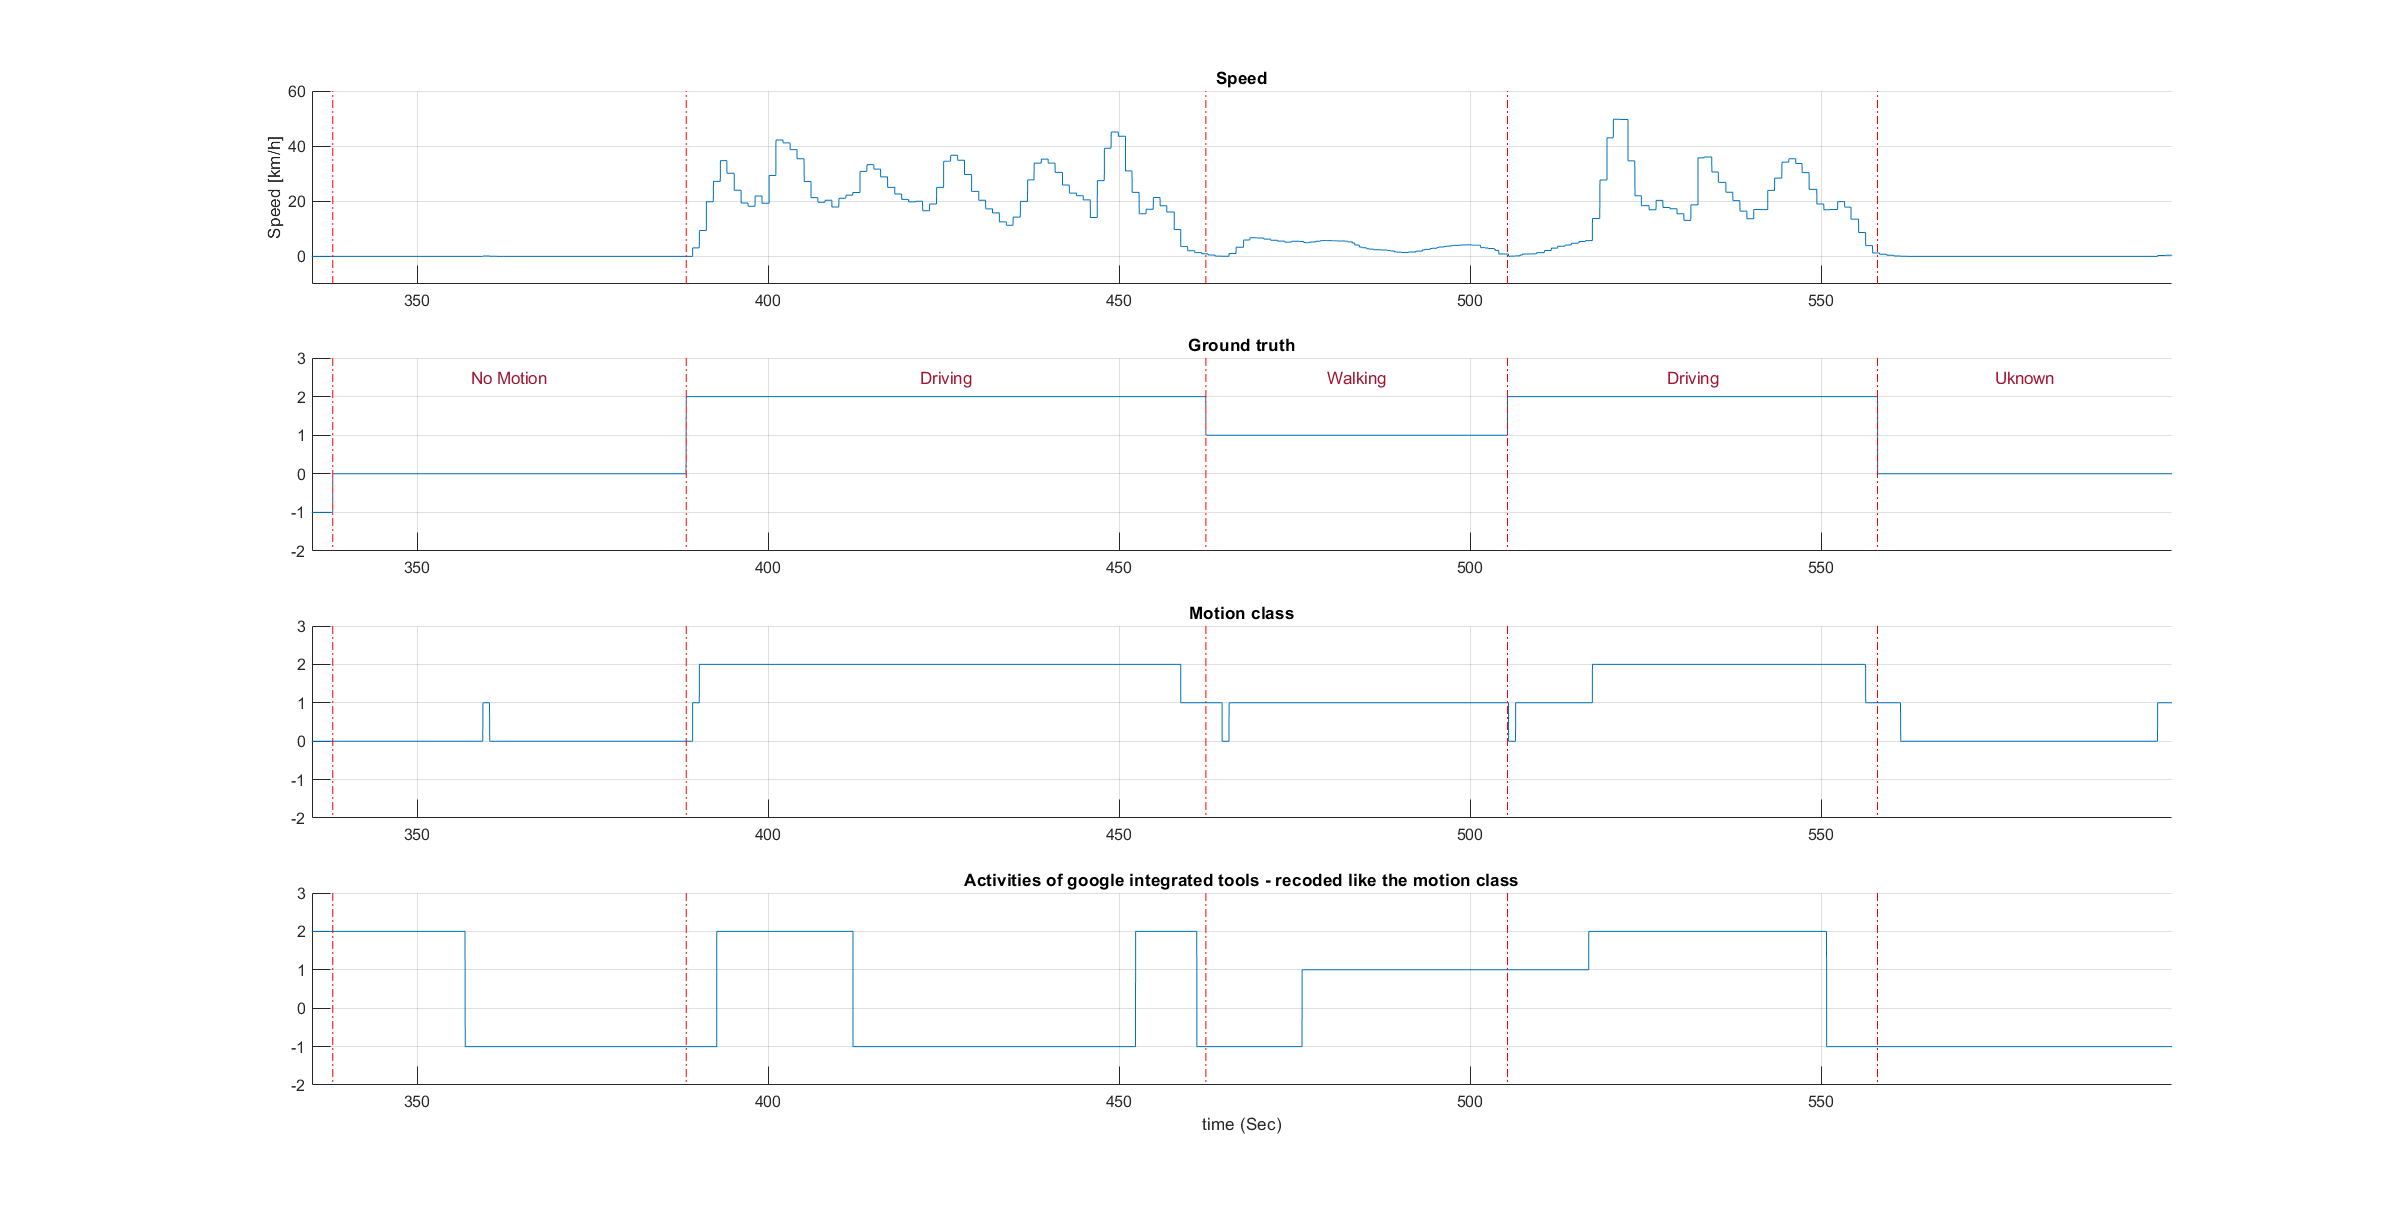
\includegraphics[width=\linewidth]{Bilder/Speed_Groundtruth_MotionClass_GoogleMD_Compare.png}
	\caption{Ergebnis des Lauferkkennungsmodells}
	\label{fig:Speed_Groundtruth_MotionClass_GoogleMD_Compare}
\end{figure}



\section{Auf und Absteigen}

\begin{figure}[H]
	\centering
	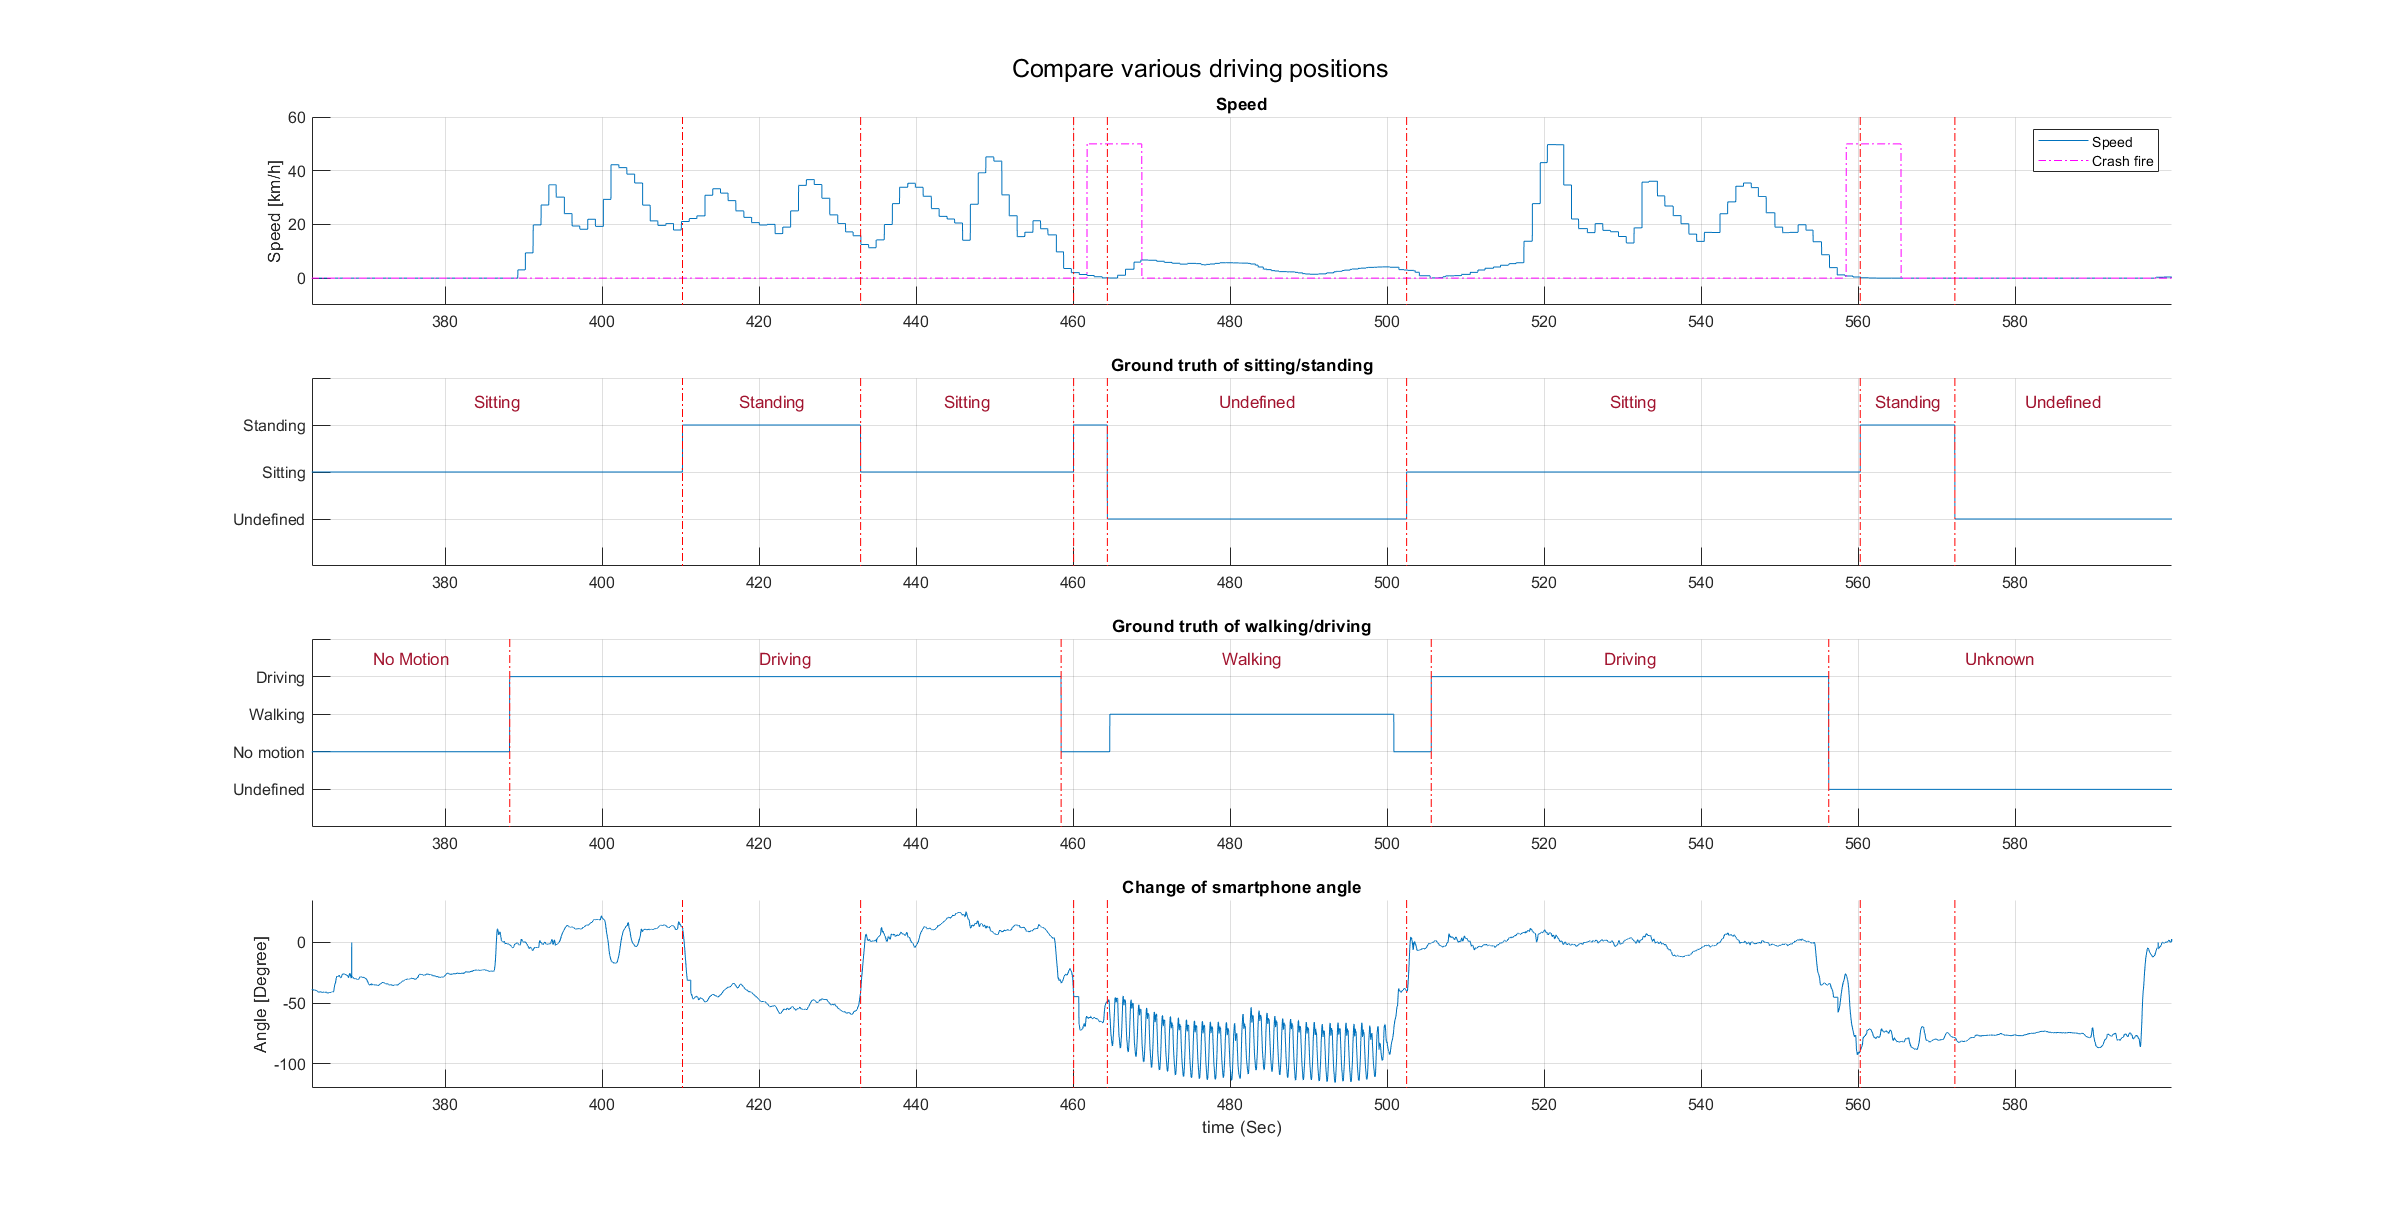
\includegraphics[width=\linewidth]{Bilder/Speed_Groundtruth_WalkStand_Compare.png}
	\caption{Vergleich der Fahrt in vertikaler und normaler Position}
	\label{fig:Speed_Groundtruth_WalkStand_Compare}
\end{figure}


\section{Verifikationsversuche}



\section{Vor- und Nachteile}
- Rechenzeit: kein wesentlicher Unterschied (55 Sec und 57 Sec)





 